
\chapter{RISC-V simulátor Jana Vávry a Jakuba Horkého}
\label{chapteroldsolution}

Tato kapitola se bude zabývat analýzou simulátoru, který byl výsledkem diplomových prací, na které navazuji \cite{horkySim, vavraSim}.
Poskytne přehled o~fungování systému, zaměří se na jednotlivé moduly a funkce simulátoru, pro které budou v~následující kapitole navržena zlepšení.

V~současném stavu má simulátor podobu desktopové aplikace s~grafickým uživatelským rozhraním.
Celý systém je implementován v~programovacím jazyce \emph{Java}\footnote{\url{https://www.java.com/en/}} s~použitím knihovny JavaFX\footnote{\url{https://openjfx.io/}}.
Aplikace nemá rozhraní příkazové řádky.

\section{Architektura systému}
% MVVM Pattern
% DI, OOP, 
% code organisation

Kód simulátoru je organizovaný do modulů.
Implementace využívá objektově orientovaného přístupu k~programování.
Třídy simulace se dělí na datové (modely) a behaviorální (jednotlivé simulované bloky).

Centrální třída simulace \texttt{BlockScheduleTask} si udržuje seznam referencí na všechny simulované bloky procesoru.
V~případě kroku simulace vpřed nebo zpět je posluchačům v~definovaném pořadí zaslaná odpovídající zpráva.
Ke komunikaci je použit návrhový vzor \emph{Observer}.

V~programu existuje globální instance stavu simulace.
Komponenty uživatelského rozhraní obdrží reference na potřebné objekty systémem založeném na návrhovém vzoru vkládání závislostí (Dependency Injection).

Každý komponent uživatelského rozhraní má své třídy \emph{view} a \emph{controler}, které definují vzhled a chování podle archtektury MVVM.
% todo check

\section{Interpretace instrukcí}
\label{interpret}

Každá instrukce z~instrukční sady je popsána několika atributy.
Výpis \ref{code.1} uvádí popis jedné z~instrukcí.
Definuje jméno instrukce, počet operandů a třídu instrukce (aritmetická, paměťová, skoková).
Součástí popisu je také výraz, který definuje vztah zdrojových a cílových operandů.

% listing byl nešikovně
\newpage

\begin{lstlisting}[caption={Popis instrukce \texttt{add}. Položka \texttt{interpretableAs} obsahuje matematický popis instrukce.},captionpos=b,label=code.1]
    {
      "name": "add",
      "instructionType": "kArithmetic",
      "inputDataType": "kInt",
      "outputDataType": "kInt",
      "instructionSyntax": "add rd rs1 rs2",
      "interpretableAs": "rd=rs1+rs2;"
    }
\end{lstlisting}

Tento výraz je ve fázi execute interpretován objektem představujícím příslušnou funkční jednotku.
Jedná se o~interpret s~precedenční analýzou operátorů.
Implementace obsahuje precedenční tabulku a operátor přiřazení řeší zvlášť.

Každý druh operace má svůj vlastní interpret (\texttt{Code\-Load\-Store\-Interpreter}, \texttt{Code\-Branch\-Interpreter}, \texttt{Code\-Arithmetic\-Interpreter}).
Důvodem jsou odlišné požadavky na popis a vykonání těchto instrukcí.

Tento přístup má své výhody i nevýhody.
Nespornou výhodou je možnost definovat nové instrukce pouhou úpravou konfiguračních souborů.
Jako nevýhody vnímám nižší výkon simulace a vyšší složitost kódu.

Interpret a jeho jazyk není dostatečně silný pro vyjádření některých instrukcí, případně pseudoinstrukcí s~implicitními argumenty.
Některé informace o~instrukcích jako například cíl skoku, nebo cílový registr jsou vyjádřeny implicitně.
Implementace nepopisuje všechny instrukce základní instrukční sady, zato ale implementuje část rozšíření M pro násobení a rozšíření F pro čísla s~plovoucí desetinnou čárkou.
% nepopisuje žádné pseudoinstrukce

% https://github.com/riscv-non-isa/riscv-asm-manual/blob/master/riscv-asm.md#-a-listing-of-standard-risc-v-pseudoinstructions
Syntax assembleru je nestandardní, není kompatibilní s~assemblerem generovaným rozšířenými překladači jako GCC.
Důsledkem je, že programy vytvořené překladačem nebo nalezené na internetu musí být před spuštěním upraveny.
Nejsou podporovány žádné direktivy pro definování globálních dat.

\section{Konfigurace simulace}

V~uživatelském rozhraní simulátoru lze konfigurovat velikosti bufferů, chování cache a prediktoru skoků.

Lze také konfigurovat množství a latence jednotlivých funkčních jednotek.
Konfigurace ALU spočívá v~definování povolených operací jazyka pro popis instrukcí zmíněného v~sekci \ref{interpret}.
Chybí zde konfigurace latence konkrétních operací.
Například operace dělení typicky trvá výrazně více taktů, než sčítání.

Simulace má více konfiguračních možností v~podobě souborů JSON, které definují instrukce (viz ukázka \ref{code.1} v~sekci \ref{interpret}) a registry.
Tuto konfiguraci není nutné poskytovat uživatelům, protože pro instrukční sadu RISC-V jsou instrukce a registry přesně definovány. 

\section{Zpětná simulace}

Značná část složitosti celého systému spočívá v~možnosti krokovat simulaci dopředu i zpět v~čase.
Tato funkcionalita je dosažena tím způsobem, že každý funkční blok implementuje krok v~čase o~takt dopředu (\texttt{simulate}) a inverzní operaci (\texttt{simulateBackwards}).

Každá změna stavu musí být reverzibilní, stav procesoru musí držet celou svou historií a proto  s~délkou simulace velikost stavu značně roste.
Simulace například udržuje seznam všech vydaných instrukcí a historii všech paměťových transakcí.
Dostatečně dlouhá simulace musí nutně vést k~vyčerpání zdrojů.

\section{Reprezentace registrů}
\label{repr_reg}

Registry jsou organizovány do skupin podle datového typu (integer a float).
V~těchto skupinách jsou i zobrazované v~uživatelském rozhraní, spekulativní registry zobrazené nejsou.

Číselné hodnoty jako stavy registrů a mezivýpočty při interpretaci jsou reprezentovány výhradně v~datovém typu \texttt{double}.
Tento datový typ neodpovídá chápání registrů v~architektuře RISC-V, která s~registry pracuje jako s~bitovým polem.

Používání \texttt{double} pro reprezentaci registrů má několik implikací:
\begin{itemize}
    \item grafické rozhraní nemá dostatek informaci pro interpretaci obsahu registru a proto ho musí zobrazit jako desetinné číslo, a to i v~případech, kdy je význam obsahu jiný (celé číslo, pravdivostní hodnota, ukazatel),
    \item interpretace celočíselných instrukcí musí provádět přetypování před a po výpočtu,
    \item přesnost simulace je nedostatečná -- tento nedostatek je nejzřetelnější u~výsledků bitových operací.
\end{itemize}

\section{GUI}

Hlavní okno simulátoru (na obrázku \ref{old_gui}) poskytuje vhled do stavu celého procesoru a prvky k~ovládání simulace.
Kód, registry a buffery jsou reprezentovány tabulkami.
Horní lišta umožňuje spustit celou simulaci, nebo ji postupně krokovat.
Čáry mezi jednotkami procesoru znázorňují datové cesty.

Celé znázornění procesoru se nevejde do jednoho okna, k~prohlédnutí některých částí je nutné okno posunout posuvníkem.
Pro pohled do cache a na statistiky jsou vyhrazena speciální okna přístupná z~pravé lišty.
V~horní části obrazovky se nacházejí tlačítka pro přechod do editoru kódu a nastavení parametrů simulace.

\begin{figure}[hbtp]
    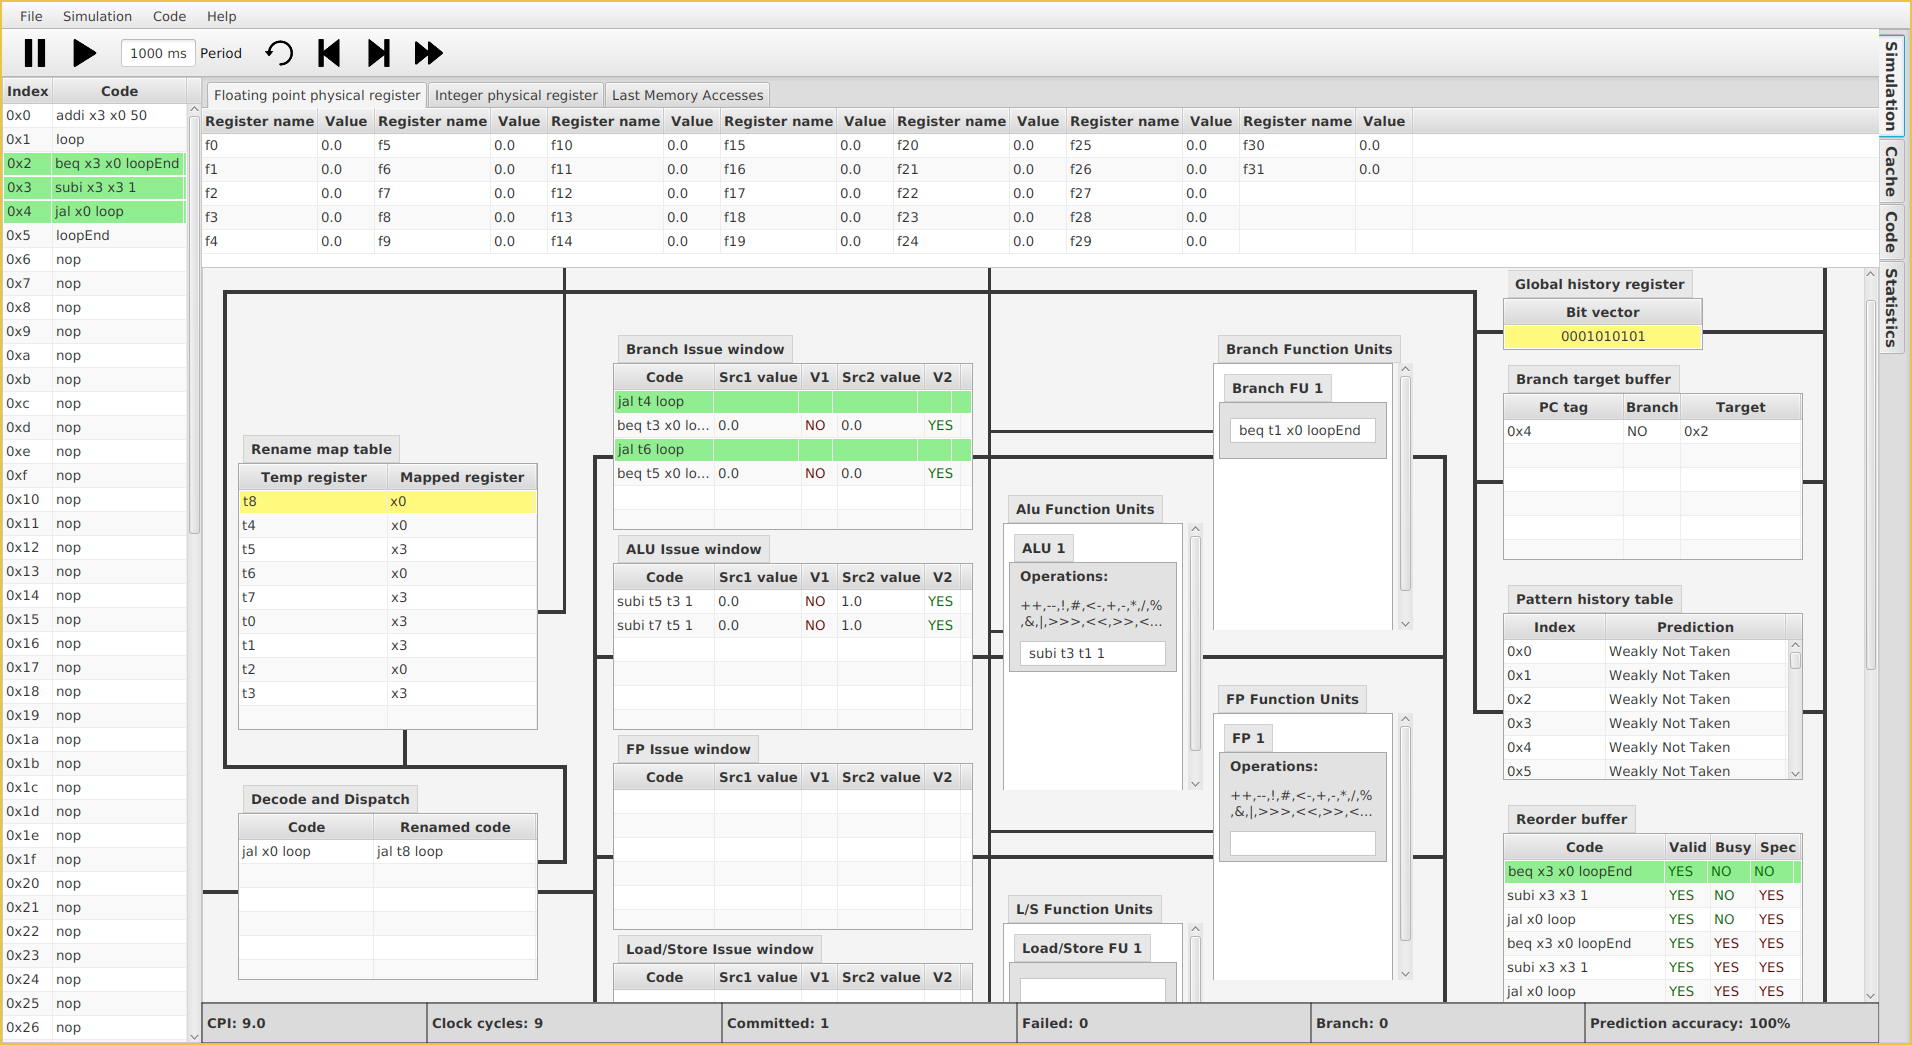
\includegraphics[width=\textwidth]{obrazky-figures/simulating.png}
    \caption{Hlavní okno původní aplikace v~průběhu simulace. \cite{horkySim, vavraSim}}
    \label{old_gui}
\end{figure}

\subsection{Statistiky}

Vybrané statistiky jsou zobrazeny v~dolní části hlavního simulačního okna (obrázek \ref{old_gui}).
Detailnější pohled poskytuje záložka \emph{Statistics}, kterou je možné vidět na obrázku \ref{stat_window}.
Zde se nachází více číselných statistik a dva grafy vývoje statistik v~čase.
Tabulka ve spodní části obrazovky se rozšíří o druhý řádek se statistikami.

\begin{figure}[hbtp]
    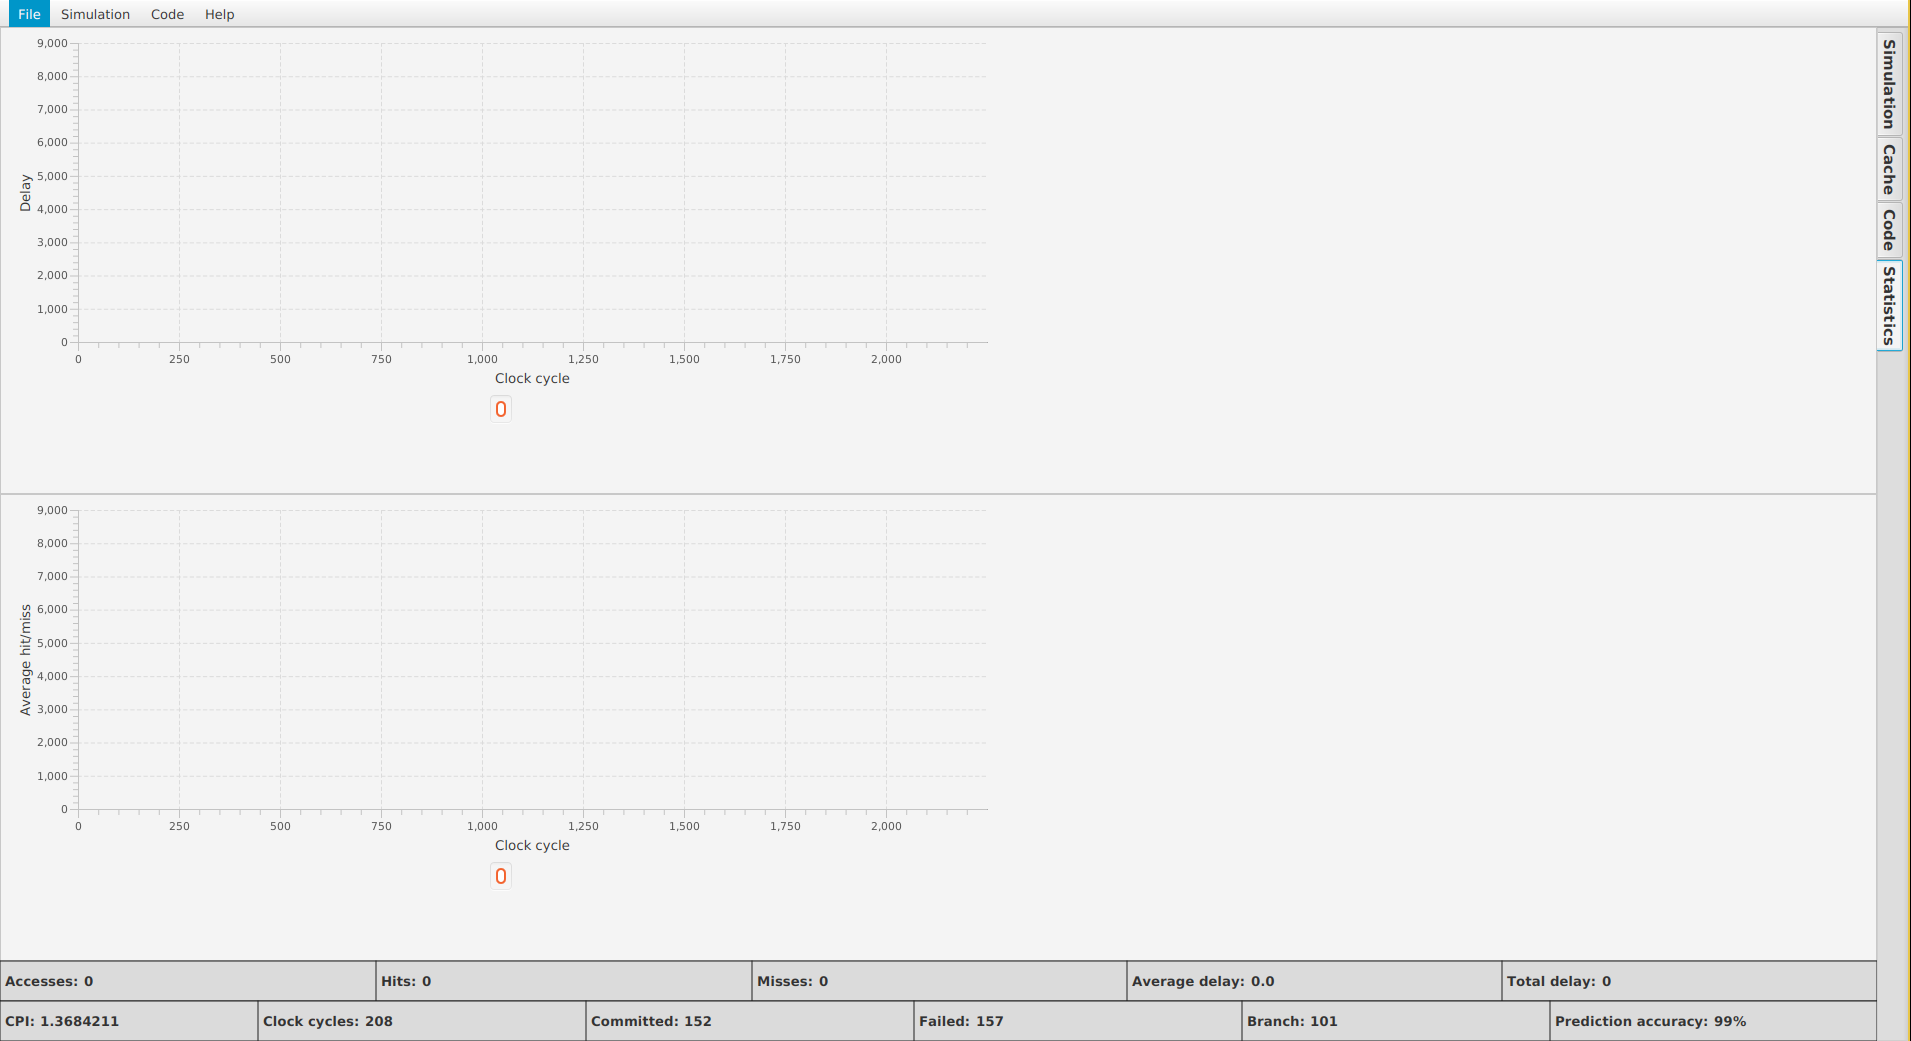
\includegraphics[width=\textwidth]{obrazky-figures/stats.png}
    \caption{Okno pro zobrazení statistik simulace. \cite{horkySim, vavraSim}}
    \label{stat_window}
\end{figure}

Chybí mi zde více statistik, například instrukční mix (poměr typů instrukcí v~kódu), nebo vytíženost funkčních jednotek.
Prezentace statistik také není příliš názorná.

\section{Editor kódu a kompilátor}
\label{inhouse_compiler}

Aplikace umožňuje vytvářet vlastní kódy v~assembleru RISC-V, nebo v~jazyce C, který je do assembleru následně přeložen.
Kód lze následně přenést do simulátoru.

Editor (na obrázku \ref{code_window}) je praktický.
Je možné nahrát jeden z~mnoha předpřipravených příkladů kódu, což snižuje úsilí nutné k~vyzkoušení simulátoru.
Zajímavou vlastností je vizualizace vztahu mezi kódem v~jazyce C a assemblerem v~podobě zvýraznění řádků programů.

\begin{figure}[hbtp]
    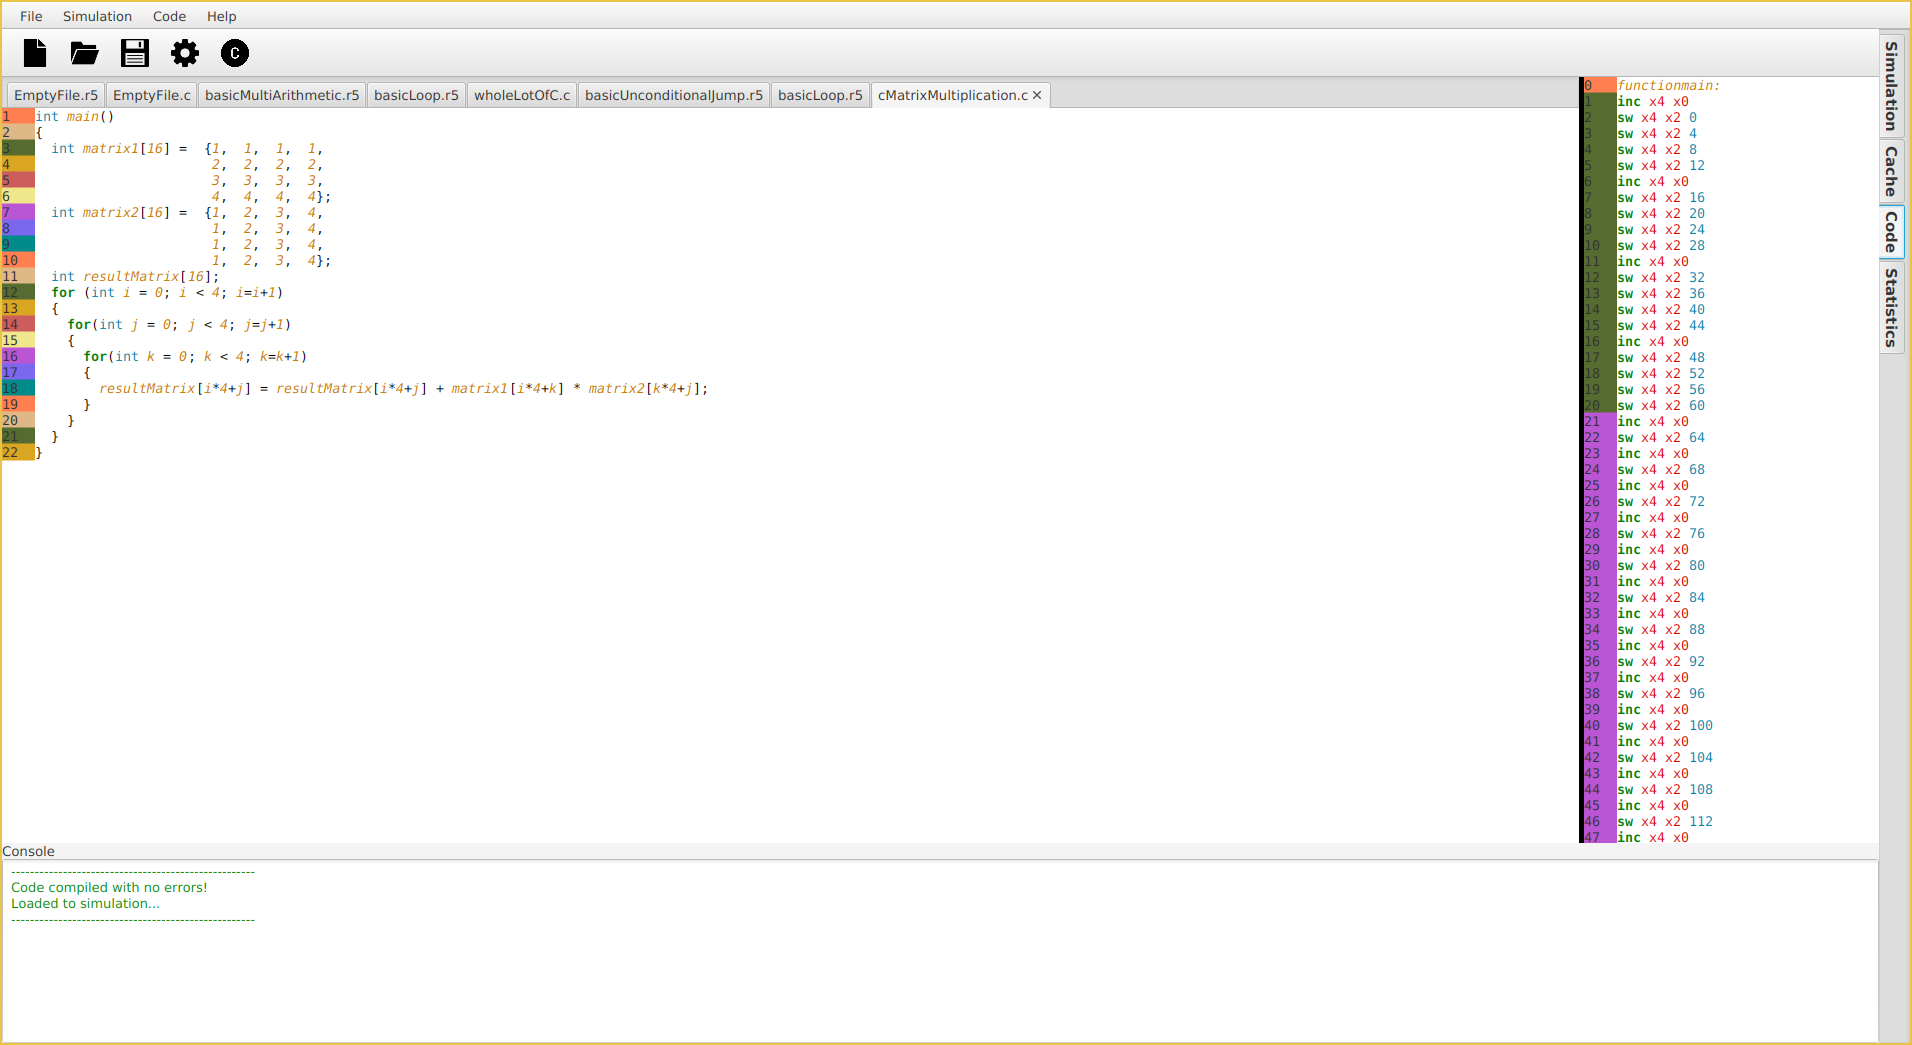
\includegraphics[width=\textwidth]{obrazky-figures/codeeditor.png}
    \caption{Editor kódu zabudovaný v~původní aplikaci.}
    \label{code_window}
\end{figure}

Mít překlad plně pod svou kontrolou je velkou výhodou, zejména pokud simulátor nepodporuje všechny instrukce a direktivy, které běžný překladač může vygenerovat, nebo pokud se syntax odchyluje od standardu.
Udržovat vlastní překladač jako součást simulátoru ale považuji za velkou zátěž.
Vyladit všechny chyby je příliš těžké, zpětná vazba kompilátoru v~podobě chybových hlášení jsou obecná.
Absence podpory celého standardu C znamená, že kód stažený z~internetu často nemusí fungovat.
Uživatel navíc nezná limity překladače, což znesnadňuje práci.

Jediným způsobem jak definovat data je jako jednorozměrné pole v~lokální proměnné ve funkci přímo v~kódu.
Taková definice dat se navíc přeloží jako série instrukcí \texttt{store} uvnitř těla funkce, což funkci učiní méně čitelnou a zanese šum do běhových statistik programu.

\section{Testování}

Testování je v~projektu na skvělé úrovni.
Dobře pokrývá jednotlivé moduly i celkové chování simulátoru, čímž napomáhá snadnějšímu pochopení kódu a ulehčuje refaktorizaci a implementaci nové funkčnosti.

Projekt používá testovací framework JUnit. % https://junit.org/junit5/

Jakub Horký zmiňuje \cite{horkySim}, že implementací nových funkcí musel velkou část testů opravovat.
Z~mých experimentů mám podobné zkušenosti, zejména se jedná o~holistické testy, které vynucují přesný stav simulace v~každém kroku. 

\chapter{Návrh rozšíření simulátoru}
\label{navrhrozsirenisimulatoru}

V~této kapitole se budu zabývat návrhem rozšíření simulátoru na základě analýzy z~předchozí kapitoly.
Navrhnu změnu architektury na serverovou s~webovým klientem.
Vylepšení se zaměří na dva aspekty, 1) uživatelské rozhraní a 2) přesnost simulace.

Musí být zachována dobrá rozšiřitelnost a modularita simulátoru.
Implementace by měla v~případě budoucího rozšíření povolit nenáročné rozšíření o~další část instrukční sady, nebo funkční blok jako například vektorová jednotka.

Při návrhu uživatelského rozhraní jsem se inspiroval původním rozhraním simulátoru Jana Vávry a Jakuba Horkého.
Programátorská rozšíření stavěla na objektové struktuře původního návrhu.

\section{Architektura systému}
% servery, klienti, deployment

Desktopovou aplikaci s~grafickým uživatelským rozhraním přetvořím na HTTP server s~bezstavovým aplikačním rozhraním využívající HTTP a rozhraním pro lokální práci v~příkazové řádce.

HTTP API bude využívat nová klientská webová aplikace.
Ta bude implementovat pouze zobrazení stavu procesoru, editování kódu a konfiguraci simulace.
Vytvořením samostatně stojící prezentační vrstvy získává projekt možnost tyto dva systémy nezávisle nasazovat, udržovat a případně znovu implementovat.

Rozhraní příkazové řádky bude sloužit k~automatizovanému spouštění simulací.

\subsection{Webové technologie}

Poskytování uživatelských rozhraní pomocí webového prohlížeče má značné výhody.
Uživatel nemusí plnit složité požadavky na hardwarovou a softwarovou výbavu nutnou k~instalaci a spuštění softwaru.
Většina uživatelů již má počítač s~moderním webovým prohlížečem a internetové připojení.
% TODO data, zdroj. Kolik procent lidí/počítačů tím disponuje

Vzhledem k~původní implementaci v~jazyce Java se nabízí možnost implementovat renderování webového uživatelského rozhraní jako modul.
Java k~takovým účelům dokonce poskytuje rámcová řešení.
Zachování monolitické povahy simulátoru by bylo výhodou, aplikace ale kvůli požadavkům na názornost a interaktivitu bude vyžadovat značné množství logiky na straně klienta.
% Proč je to výhodné

Ekosystém pro návrh a implementaci front-endových aplikací pomocí JavaScriptu je značně vyspělý.
Z~těchto důvodů jsem se rozhodl klientskou aplikaci vyvinout s~knihovnou React a frameworkem NextJS.
Při vývoji budu moci využít existující ekosystém pokročilých nástrojů a mnoha knihoven.

\subsection{Aplikační rozhraní}
\label{httpapidesign}

Simulátor a webová aplikace budou komunikovat pomocí protokolu HTTP aplikačním rozhraním založeným na formátu JSON. 

Stav navracený ze simulátoru by měl být \emph{normalizovaný}.
Simulátor jakožto objektově orientovaný program pracuje s~grafem navzájem se odkazujících objektů.
Serializace takového grafu do hloubky způsobí zacyklení.
Navíc, nenormalizovaná data znamenají redundanci v~podobě kopií.
Normalizace datových objektů proběhne nahrazením referencí za identifikátory v~době serializace.

% Rizika: latence
Možným rizikem je latence serveru při interaktivní simulaci.
Při vývoji a hodnocení budu tuto metriku sledovat a v~případě nevyhovujících parametrů implementuji opatření.

\section{Jednotlivá vylepšení simulátoru}
\label{rozsireniJava}

Kromě dále zmíněných konkrétních vylepšení obecně zvýším kvality kódu pomocí refaktorování a dokumentace.
Cílem je mít dobře čitelný, výkonnější a udržitelnější kód.

\subsection{Reprezentace hodnot registrů}

V~sekci \ref{repr_reg} jsem uvedl omezení současného systému, který hodnoty registrů reprezentuje v~datovém typu \texttt{double}. 

Navrhuji stav registru reprezentovat jako bitové pole.
Interpretace hodnoty bude záviset na právě prováděné instrukci.
Tato reprezentace dovolí přesnou simulaci všech instrukcí, včetně bitových operací.

Bitové pole bude široké 64 bitů, aby bylo připravené pro případné přidání 64 bitové instrukční sady.
V~případě implementace vektorových registrů bude nutná malá úprava

Spolu s~bitovým polem bude v~objektu registru uložena metainformace o~významu obsahu, tedy o~datovém typu registru. Zdrojem této informace bude popis instrukce, která hodnotu vytvořila.
Tato informace bude soužit pouze k~účelům zobrazování hodnoty v~GUI a při ladění, při simulaci nebude mít význam.

\subsection{Interpretace instrukcí}
\label{instructionNewDesign}

Změny v~interpretaci instrukcí úzce souvisí se změnou reprezentace hodnot registrů. Plánuji podporovat celou instrukční sadu RISC-V včetně pseudoinstrukcí. Tento cíl vyžaduje jisté další úpravy.

Navrhuji sjednotit interprety do jedné implementace, která bude dostatečná pro všechny případy užití.

Precedenční interpret nahradím interpretem výrazů v~postfixové notaci. Jeho implementace je jednodušší, výrazy nepotřebují závorky a jeho vyjadřovací síla je dostatečná.
Navíc nebude potřeba zvláštního parsování pro operaci přiřazení.

Výpočet některých instrukcí pracuje s~hodnotami, které nepatří mezi operandy dané instrukce. Typickým příkladem je použití hodnoty PC při výpočtu adresy skoku. Dalším příkladem je instrukce \texttt{jal}, která načítá hodnotu PC do registru. Další kategorií jsou pseudoinstrukce, které často mají implicitní argumenty. Jako příklad uvedu pseudoinstrukci \texttt{ret}, která odpovídá instrukci \texttt{jalr x0, x1, 0}.

Funkční popis takových instrukcí vyřeším zavedením konceptu proměnných do interpretace. Popis instrukce bude obsahovat všechny argumenty a jejich datové typy. Tyto datové typy budou řídit interpretaci bitů uložených v~daných registrech.
Příklad navrhovaného popisu instrukce naleznete na obrázku \ref{code2}.

\begin{lstlisting}[caption={Nový popis instrukce \texttt{add} detailně popisuje argumenty a jejich datové typy.},captionpos=b,label=code2]
   {
    "name": "add",
    "instructionType": "kArithmetic",
    "arguments": [
      {
        "name": "rd",
        "type": "kInt",
        "writeBack": true
      },
      {
        "name": "rs1",
        "type": "kInt"
      },
      {
        "name": "rs2",
        "type": "kInt"
      }
    ],
    "interpretableAs": "\\rs1 \\rs2 + \\rd ="
  },
\end{lstlisting}


% default values, pseudoinstructions

\subsection{Rozhraní simulátoru, reprezentace stavu}

Bude odstraněno grafické uživatelské rozhraní, aplikace bude komunikovat bezstavově schématem požadavek/odpověď.
Požadavek bude moct být podán prostřednictvím příkazové řádky (CLI), nebo HTTP dotazu.

Hlavním požadavkem bude dotaz na stav simulace v~určitém kroku pro určitou konfiguraci procesoru.
Výstupem bude stav procesoru, statistiky o~běhu a ladící výstupy.

Další možné požadavky na simulátor budou:
\begin{itemize}
    \item překlad programu z~jazyka C do assembly,
    \item kontrola správnosti programu v~assembly,
    \item kontrola správnosti konfigurace CPU pro simulaci.
\end{itemize}

% Požadavky na CLI
Simulace spouštěná z~příkazové řádky přijme jako argument konfiguraci procesoru, včetně simulovaného programu.
Výstupem budou především statistiky o~dokončeném běhu.
Rozhraní příkazové řádky je určeno primárně pro hromadné vyhodnocování, nebude umožňovat interaktivní simulování, ani překlad programů v~jazyce C.

% HTTP
% velikost zpráv, endpointy
HTTP API bude očekávat \texttt{POST} dotazy s~parametry předávanými v~těle zprávy v~jazyce JSON.
Odpovědi budou také v~jazyce JSON.
Jazyk JSON jsem zvolil kvůli dobré podpoře jeho zpracování ve webových aplikacích.
Stav procesoru může být objemný, proto plánuji podporovat kódování ZIP, které významně sníží množství dat přenášené po síti.

Dalším problémem je serializace stavu procesoru.
Stav má strukturu obecného grafu objektů s~mnoha cykly, které JSON není schopen nativně vyjádřit.
Řešením bude stav normalizovat, převést ho z~obecného grafu do stromu a chybějící hrany vyjádřit implicitně identifikátory. 

V~současné podobě aplikace nemůže existovat více instancí procesoru.
Stav procesoru bude muset být přesunut do rodičovského objektu, který bude obsahovat reference na všechny své komponenty.

\subsection{Zpětná simulace}
\label{backSimNewDesign}

Aby bylo možné realizovat zpětnou simulaci bezstavovými dotazy podle současné implementace, musel by být stav procesoru přenášen spolu s~dotazem.
Na tento stav by se pak aplikoval krok dopředu nebo zpět.
Logika zpětné simulace je zároveň velmi složitá, výrazně zvětšuje velikost stavu a obsahuje těžko odhalitelné chyby.

Navrhuji zcela jiný přístup.
Simulace bude probíhat \emph{pouze} ve směru dopředu v~čase.
Dotaz bude obsahovat počáteční konfiguraci (kód a vlastnosti procesoru) a požadovaný takt $t$.
Simulátor provede $t$ kroků z~času $0$ do času $t$ a stav simulace vrátí.

Interaktivní simulace funguje na principu dotazu na stav $t-1$ nebo $t+1$.
Jinými slovy zpětná simulace může být realizována dopřednou simulací z~výchozího stavu.
Dotaz tedy nemusí přenášet stav simulace, ale pouze počáteční konfiguraci.
To je výhodné z~pohledu množství přenášených dat po síti.

Pro lepší ilustraci uvedu konkrétní příklad.
Předpokládejme situaci, kdy uživatel provozuje interaktivní simulaci a nachází se na 20. taktu.
Pokud uživatel požádá o~krok zpět (stav v~taktu 19), spustí se simulace z~výchozího stavu (stav v~taktu 0) a provede se 19 kroků simulace vpřed.

Předpokladem je, že je simulace deterministická.
Rizikem tohoto přístupu je latence při interaktivní simulaci -- délka výpočtu následujícího stavu bude růst s~aktuální pozicí simulace v~čase, protože celá simulace musí proběhnout znovu.
V~případě, že odpověď serveru nebude spolehlivě dosahovat interaktivní rychlosti, je možné implementovat cache a stavy spekulativně předpočítávat.
% Obsloužení dotazu bude mít stále konstantní cenu.

\subsection{Přesnost simulace}
% labels - návěstí, instruction set, tests, Expression

Mým cílem je implementovat všechny instrukce základní instrukční sady RV32I a rozšíření M a F.
Výjimkou budou instrukce pro komunikaci s~jádrem, protože není implementovaný privilegovaný režim ani přepínání kontextu.
Implementuji i velkou část pseudoinstrukcí.

Každá z~instrukcí bude přesně odpovídat specifikaci.
Instrukce programu ale budou i nadále vnitřně reprezentovány polem objektů, nebudou zavedeny a čteny z~paměti.

Skokové a paměťové operace pracují s~adresami návěstí.
V~současné implementaci ale hodnota návěstí představuje index do pole instrukcí.
Návěstím je nutné přiřadit reálné adresy, aby hodnoty odpovídaly očekávání překladače a aby mohly návěstí ukazovat na staticky alokovaná pole a konstanty (více v~sekci \ref{memloader}).

\subsection{Konfigurace simulace}

Stávající konfigurace je převážně vyhovující.
Hlavní změnou konfigurace jádra bude zjednodušení konfigurace ALU.
Místo seznamu operací si uživatel bude moci vybrat jednu nebo více z~pěti funkcionalit: sčítací operace, bitové operace, násobení, dělení a speciální funkce.

V~GUI přidám detailní popisy ke každé možnosti konfigurace, aby bylo zřejmé jaký efekt má na simulaci.
Přibude i validace vstupů s~dobrou zpětnou vazbou pro uživatele.

Novou funkcí bude definice paměťových míst přímo v~konfiguraci.
Je užitečné sledovat běh algoritmů na určitých datech, například některá chování cache se projeví až při práci s~větším množstvím (kilobajty) dat
Navrhuji přidat možnost pohodlně definovat větší datové vstupy položkami v~aplikačním dotazu (tedy jinou cestou, než direktivami v~kódu).
Paměťové místo bude definované svým názvem, datovým typem, požadavkem na zarovnání v~paměti a seznamem číselných hodnot.

\subsection{Kompilace programů v~jazyce C}

Překladače jsou jedním z~nejkomplexnějších problémů oblasti informatiky.
Proto by bylo vhodné použít hotové řešení.

Vybral jsem si překladač \emph{GCC}\footnote{\url{https://gcc.gnu.org/}}, jeden z~nejpoužívanějších překladačů pro jazyk C.
Poskytuje užitečná chybová hlášení, je dobře otestovaný, rychlý a implementuje veškeré potřebné funkce jazyka C.

GCC má mnoho funkcí a obsáhlou dokumentaci.
Plánuji uživatelům zpřístupnit ovládání optimalizací.
Bude také možné si vyzkoušet efekt direktiv jako \texttt{\#pragma unroll}. 

Tento překladač podporuje \emph{cross-compilation}, kompilaci pro jinou architekturu, než ta, na kterém je překladač spouštěn.

Překladač bude front-endové aplikaci zpřístupněn jako součást simulačního API. 
Serverová aplikace bude binární program GCC spouštět přes shell se zvolenými přepínači.
Řetězec s~programem bude poslán na jeho standardní vstup, z~výstupu bude přečten assembler pro RISC-V.
Chybová hlášení budou předána zpět uživateli webového editoru.

Překladač generuje jiný kód, než jaký v~současnosti překladač očekává.
Změny, které musím implementovat zahrnují:
\begin{itemize}
    \item změnu syntaxe (viz sekce \ref{riscvSyntax}),
    \item přidání podpory pro aliasy registrů,
    \item implementaci všech instrukcí, které překladač může generovat,
    \item alokaci zásobníku volání (viz sekce \ref{memloader})
    \item zastavení simulace při vyprázdnění zásobníku volání,
    \item filtrování ladících symbolů a nepoužitých direktiv.
\end{itemize}

\subsection{Syntax programů v~asembleru RISC-V}
\label{riscvSyntax}

Protože plánuji používat klasický překladač, budu muset simulátor upravit tak, aby přijímal tradiční assembler RISC-V.
To znamená především:
\begin{itemize}
    \item přidání oddělovačů mezi parametry (čárky a závorky),
    \item parsování direktiv (například \texttt{.word}),
    \item implicitní paramtery (pro pseudoinstrukce).
\end{itemize}

Ladící výstupy budou realizovány komentáři, takže neovlivní syntax assembleru.

\subsection{Sběr statistik o~běhu}
\label{statsCollection}

Sběr statistik bude detailnější.
Zaměřím se jak na globální statistiky, tak i statistiky jednotlivých instrukcí.

Konkrétní návrhy nových statistik:
\begin{itemize}
    \item statický a dynamický instrukční mix,
    \item vytíženost každé funkční jednotky,
    \item počty provedení každé instrukce,
    \item nové charakteristiky (FLOPS, aritmetická intenzita).
\end{itemize}

Se statistikami tečně souvisí sběr ladících zpráv.
Při vytváření programu bude možné k~libovolné instrukci přidat komentář ve speciálním formátu se zprávou.
Při potvrzení instrukce s~ladící zprávou bude zpráva přidána do logu.
Zpráva umožní vložení aktuální hodnoty registrů.
Bude také zaznamenána časová známka zprávy, která bude prezentována vedle zprávy v~uživatelském rozhranní.

\subsection{Zavádění dat do paměti procesu}
\label{memloader}

Data definovaná v~konfiguraci i v~assembleru direktivami\footnote{Jako příklad, \texttt{A: .word 1,2,3,4} definuje pole \texttt{A} o~čtyřech 32 bitových prvcích.} musí být staticky alokována v~hlavní paměti procesoru.
Alokace proběhne podle požadavků na datový typ a \emph{zarovnání}.

Program v~jazyce C bude přeložen do direktiv.
Tímto způsobem bude možné alokovat globální proměnné, včetně struktur a řetězců definovaných v~jazyce C.

Kód s~pamětí následně bude pracovat pomocí návěstí (labels), která do této doby byla používaná pouze pro adresy skoků.
Hodnoty návěstí budou představovat ukazatele na tato pole.
% návěstí nebo label nebo?

% alokace zásobníku volání
ABI používané překladačem počítá s~alokovaným zásobníkem volání.
Proto inicializace paměti musí vyhradit místo pro zásobník a zapsat ukazatel do registru \texttt{x2} (neboli \texttt{sp}).

Příklad rozložení zásobníku volání a dvou polí se zarovnáním lze vidět na obrázku \ref{memlayout_schema}.
Počáteční adresy jsou vyhrazeny pro zásobník volání, poté jsou alokována jednotlivá pole.
Prázdné místo mezi bloky (zvýrazněno jako \emph{(a)} může vznikat požadavkem na zarovnání počátku pole v~paměti.

\begin{figure}[hbtp]
\centering
    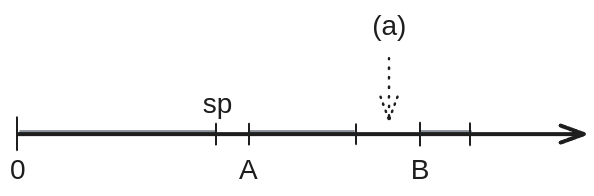
\includegraphics[width=13cm]{obrazky-figures/memlayout.png}
    \caption{Schéma rozložení dat v~paměti procesoru.} 
    \label{memlayout_schema}
\end{figure}

\section{Návrh webové aplikace}
\label{webAppDesign}
% Rozhraní simulátoru
% GUI

Webová aplikace bude víceoknová (\emph{Multi Page Application}) s rozhraním v~anglickém jazyce.
Vícejazyčná podpora vyžaduje mnoho práce, i za použití internacionalizačních knihoven jako \texttt{i18next}.
Cílová skupina aplikace je globální a angličtina dovolí projekt používat v~mezinárodním prostředí. 
Studenti informatiky často angličtinu ovládají na dobré úrovni.
Pro studium vysokoškolského kurzu AVS je angličtina předpokladem.

Obrázek \ref{main_view_design} schématicky naznačuje možný vzhled hlavního simulačního okna.
Myšlenka současného rozhraní se nemění -- jednotlivé bloky procesoru jsou reprezentovány odpovídajícími komponenty, související bloky jsou spojeny čarami, které představují datové cesty procesoru.

\begin{figure}[ht]
    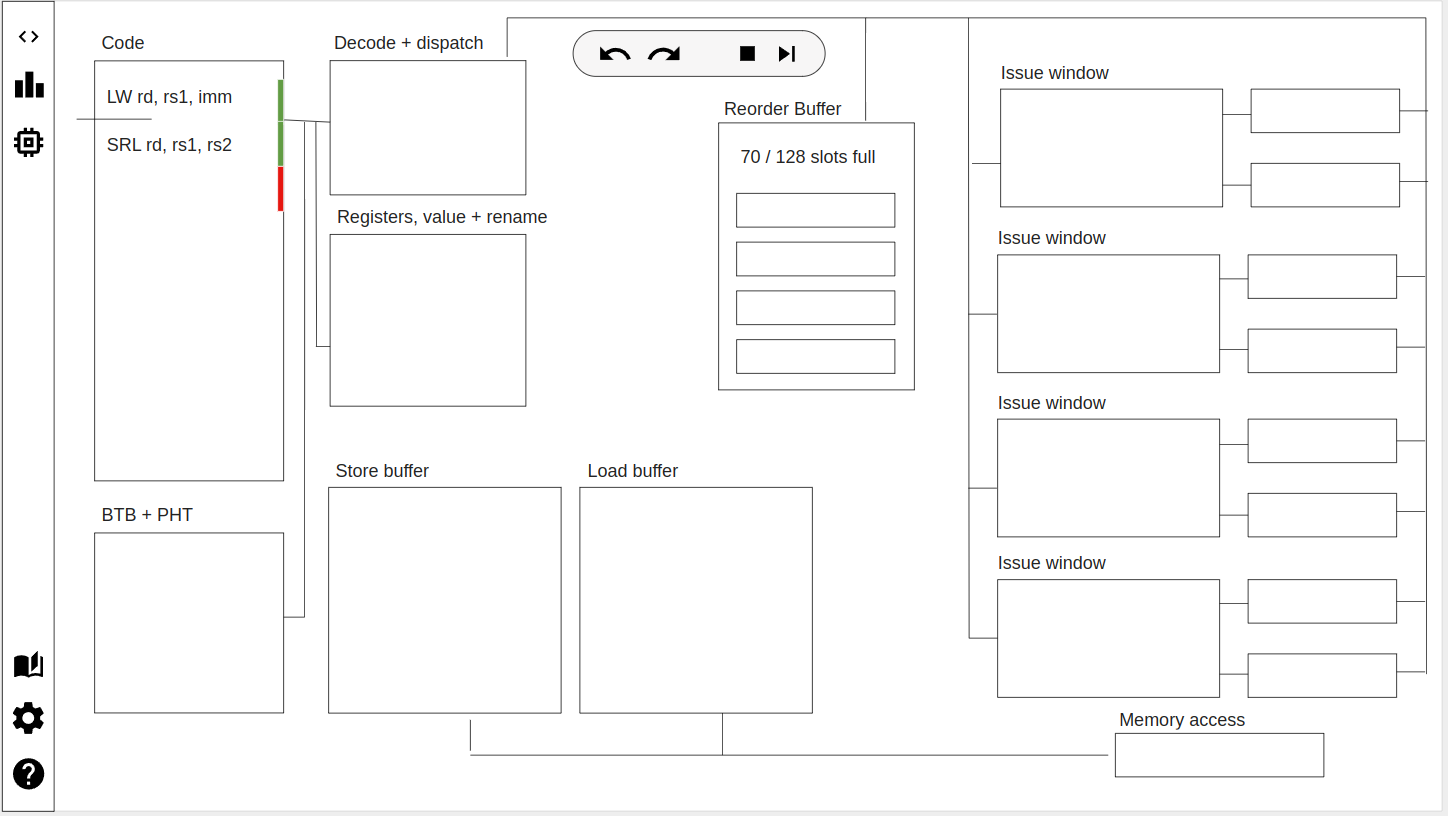
\includegraphics[width=\textwidth]{obrazky-figures/main_view_design.png}
    \caption{Schéma grafické reprezentace stavu simulace.}
    \label{main_view_design}
\end{figure}

Bloky simulace i jednotlivé instrukce by měly mít možnost detailnějšího náhledu.
Ten by kromě detailních dat měl poskytnout odkaz na dokumentaci dané instrukce nebo bloku.

Další část, která se příliš nezmění, bude ovládání simulace.
V~horní části obrazovky budou k~dispozici tlačítka pro krokování a dokončení simulace.
Pro větší komfort a dostupnost bude možné simulaci ovládat klávesnicí.

Nebude nutné uchovávat žádné uživatelské informace, nebude vyžadována ani autentizace přihlášením.
Tím odpadá nutnost jakékoliv centrální databáze a řešení souladu s regulacemi.
Konfigurace aplikace bude uložena v~lokálním úložišti prohlížeče.

\subsection{Editor kódu}
% Co je pro uživatele důležité - feedback

Záložka pro editování kódu bude umožňovat vytváření a upravování kódu v~jazyce C a v~assembleru RISC-V.

Cílem je při psaní kódu poskytnout dobrou zpětnou vazbu.
Editor bude využívat API simulátoru pro překlad a kontrolu kódu z~jazyka C do assembleru.
Případné chyby budou v~textovém poli znázorněny.
Vztah částí kódu původního a přeloženého programu bude graficky vizualizován.

K~dispozici bude několik příkladů kódů, jak pro jazyk C tak Assembler.
Příklady umožní novým uživatelům rychle začít se simulátorem experimentovat.

Vytvoření dat pro simulaci bude probíhat na jiné stránce, ale uživateli by měly být poskytnuty potřebné informace v~samotném editoru.  

\subsection{Výukové materiály}
% Texty vysvětlující RISC-V, jednotlivé bloky procesoru

Cílovými uživateli aplikace budou studenti informatiky, především kurzu AVS.
Aplikace nebude předpokládat znalost instrukční sady jako prerekvizitu, proto bude poskytovat základní informace o~instrukční sadě RISC-V v~podobě vysvětlujícího textu a tabulek.
Popis může používat odborné termíny a může se opřít o~obecné znalosti z~oblasti programování a jazyka C.

\subsection{Konfigurační stránka}
% uložit konfigurace

Konfigurace obsahuje mnoho položek, proto její vytvoření může zabrat čas a bránit od plynulého používání aplikace.
Aplikace by proto měla poskytnout rozumný výchozí profil, který by byl vyhovující pro širokou škálu experimentů.

Z~vlastní zkušenosti při experimentech s~existující konfigurací simulátoru vím, že může být obtížné představit si pod názvem konfiguračního pole jeho efekt na simulaci.
Budu klást důraz na kvalitu jmen a popisů jednotlivých polí formulářů.

Všechny vytvořené konfigurace budou uloženy lokálně v~úložišti prohlížeče a budou perzistovány napříč sezeními.
Tímto návrhem se vyhnu nutnosti spravovat uživatele v~databázi.
Alternativním přístupem by mohlo být použití autentizace a uložení dat aplikace externí službou.
Lokální úložiště je však dostatečnou a nekomplikovanou variantou.
% todo jak je na tom localstorage a gdpr, cookies zákony 

\subsubsection{Definice dat}

Pro definici simulačních dat (paměti) bude vyhrazena zvláštní sekce konfigurace. 
Uživatel bude moci definovat libovolný počet pojmenovaných paměťových lokací, na které se tímto jménem bude odkazovat v~kódu.

Počet prvků paměťového místa bude konfigurovatelný.
Hodnoty jednotlivých prvků budou inicializovány jedním ze tří způsobů:
\begin{enumerate}
    \item kopírováním konstanty,
    \item náhodnými daty,
    \item daty ze souboru CSV.
\end{enumerate}

\subsection{Prezentace statistik}

V~průběhu simulace bude možné nahlédnout na stránku se statistikami.
Zde budou prezentovány běhové statistiky popsané v~sekci \ref{statsCollection}.
Stránka poskytne přesná tabulková data i jejich vizualizaci, například teplotní mapou a grafy. 

Statistiky týkající se konkrétních bloků budou také přístupné z~jejich detailního pohledu ve \uv{vyskakovacím okně}. 

\section{Případy užití a kritéria příjmutí}
% Jak to bude testováno
% load testing
%todo

Je plánováno aplikaci využít pro výuku předmětu AVS na FIT VUT v~Brně.
Aplikace bude proto mít potenciálně stovky uživatelů.
Studenty kurzu AVS bych řadil mezi zkušené uživatele webových aplikací, nicméně bude klíčové klást důraz na intuitivnost, spolehlivost, dostupnost a výkon.

Spolehlivost aplikace ověřím dobrým automatizovaným testováním na úrovni modulů i celku.
Uživatelské rozhraní budu testovat převážně manuálně, ve dvou fázích.
Nejdříve budu testovat aplikaci v~průběhu vývoje.
Ověřím funkčnost na několika populárních internetových prohlížečích.

Později aplikaci nechám vyzkoušet několika studentům informatiky.
Při testování budu sledovat jejich práci a sbírat zpětnou vazbu.
Zpětnou vazbu využiji ke zlepšení aplikace.
Dalším zdrojem zpětné vazby je vedoucí mé práce, pan docent Jaroš, se kterým vývoj aplikace pravidelně konzultuji. 

Z~pohledu implementace je cílem co nejvyšší bezúdržbovost s~dostatečnou dokumentací pro případné drobné opravy.
Kód také může někdo v~budoucnu (stejně jako já nyní) rozšiřovat.
Klíčová bude především kvalita podpůrných dokumentů a řádně okomentovaný kód s~výstižnými jmény.

Zvážen bude i výkon aplikace.
Cílem je interaktivní simulace, proto by server měl na dotazy odpovídat do 100\,ms.
Zároveň by mělo být možné obsluhovat stovky uživatelů současně.
Splnění tohoto cíle ověřím zátěžovými testy.

Program bude pravděpodobně promítán na plátně během výuky.
Proto budu brát ohled na kontrast, možnost libovolného zvětšení prezentace simulace a na její správné škálování.
